%HW2.tex
%
% Second Homework for Graduate Algebra
% Frank Sottile
%%%%%%%%%%%%%%%%%%%%%%%%%%%%%%%%%%%%%%%%%%%%%%%%%%%%%%%%%%%%%%%%%%%%%%%
\documentclass[12pt]{article}
\usepackage{multicol,amssymb,amsmath}
\usepackage{graphicx}
\usepackage{xcolor}
\headheight=8pt
%
\topmargin=-95pt
\textheight=744pt   \textwidth=575pt
\oddsidemargin=-60pt \evensidemargin=-60pt

\pagestyle{empty}

%%%%%%%%%%%%%%%%%%%%%%%%%%%%%%%%%%%%%%%%%%%%
\newcommand{\HH}{{\mathbb H}}
\newcommand{\FF}{{\mathbb F}}
\newcommand{\RR}{{\mathbb R}}
\newcommand{\CC}{{\mathbb C}}
\newcommand{\KK}{{\mathbb K}}
\newcommand{\NN}{{\mathbb N}}
\newcommand{\TT}{{\mathbb T}}
\newcommand{\ZZ}{{\mathbb Z}}
\newcommand{\calA}{{\mathcal A}}
\newcommand{\be}{{\bf e}}

\newcommand{\Hom}{\mbox{Hom}}
\newcommand{\spec}{\mbox{spec}}
\newcommand{\cone}{\mbox{cone}}

\newcommand{\Square}{\raisebox{-2pt}{\includegraphics{figures/Square.eps}}}

\newcommand{\vect}[2]{(\begin{smallmatrix}#1\\#2\end{smallmatrix})}
\newcommand{\msp}{\hspace{8pt}}

\newcommand{\barsl}{\noindent\begin{minipage}[t]{575pt}
{\color{violet}\rule{575pt}{1.2pt}}\vspace{-5.7mm}\\
{\color{blue}\rule{575pt}{1.2pt}}\vspace{-5.7mm}\\
{\color{green}\rule{575pt}{1.2pt}}\vspace{-5.7mm}\\
{\color{yellow}\rule{575pt}{1.2pt}}\vspace{-5.7mm}\\
{\color{orange}\rule{575pt}{1.2pt}}\vspace{-5.7mm}\\
{\color{red}\rule{575pt}{1.2pt}}
\end{minipage}}


\def\demph#1{{\color{blue}{\sl #1}}}
\def\defcolor#1{{\color{blue}#1}}

\begin{document}
\LARGE 
\noindent
Algebra II\ \ Winter 2021 \hfill 25 January\makebox[40pt][l]{\ }\\
Frank Sottile \hfill
\Large\sf
Second Homework\makebox[40pt][l]{\ }\\
%\large\vspace{5pt}
\normalsize

\noindent
Write your answers neatly, in complete sentences, and prove all assertions.
Start each problem on a new page (this makes it easier in Gradescope).
Revise your work before handing it in, and submit a .pdf  created from a LaTeX source to Gradescope.
Correct and crisp proofs are greatly appreciated; oftentimes your work can be shortened and made clearer.

{\color{red}Due Monday 1 February.}\newline
\vspace{-5pt}

\barsl

\begin{enumerate}
%%%%%%%%%%%%%%%%%%%%%%%%%%%%%%%%%%%%%
%\setcounter{enumi}{52}

%%%%%%%%%%%%%%%%%%%%%%%%%%%%%%%%%%%%%%%%%%%%%%%%%%%%%%%%%%%%%%%%%%%%%%%%%%%%%%%%%
\item Let  $S:=\{1,2,2^2=4\}$, a multiplicatively closed subset of $R:=\ZZ/6\ZZ$.

  Determine (compute and identify) the ring  $R[S^{-1}]$ of fractions of $R$ by $S$.
   \vspace{-2pt} 
%%%%%%%%%%%%%%%%%%%%%%%%%%%%%%%%%%%%%%%%%%%%%%%%%%%%%%%%%%%%%%%%%%%%%%%%%%%%%%%%%


   %\newpage
%%%%%%%%%%%%%%%%%%%%%%%%%%%%%%%%%%%%%%%%%%%%%%%%%%%%%%%%%%%%%%%%%%%%%%%%%%%%%%%%%
 \item Let $R$ be a commutative ring and suppose that  $S\subset R$ is a multiplicatively closed subset (multiplicative
   subsemigroup of $R$).
   Identify the kernel of the canonical map $\iota \colon R \to R[S^{-1}]$.
   \vspace{-2pt}
%%%%%%%%%%%%%%%%%%%%%%%%%%%%%%%%%%%%%%%%%%%%%%%%%%%%%%%%%%%%%%%%%%%%%%%%%%%%%%%%%


%\newpage
%%%%%%%%%%%%%%%%%%%%%%%%%%%%%%%%%%%%%%%%%%%%%%%%%%%%%%%%%%%%%%%%%%%%%%%%%%%%%%%%%
 \item Show that for any ring $R$ and $R$-module $M$, $\Hom_R(R,M)\simeq (M,+,0)$, as abelian groups.
   \vspace{-2pt}
%%%%%%%%%%%%%%%%%%%%%%%%%%%%%%%%%%%%%%%%%%%%%%%%%%%%%%%%%%%%%%%%%%%%%%%%%%%%%%%%%

%\newpage
%%%%%%%%%%%%%%%%%%%%%%%%%%%%%%%%%%%%%%%%%%%%%%%%%%%%%%%%%%%%%%%%%%%%%%%%%%%%%%%%%
 \item  Let $R$ be a ring and $A$ be an abelian group.
   For $r\in R$ and $f\in\Hom_{\ZZ}(R,A)$, define $r.f\colon R\to A$ by $(r.f)(x)=f(xr)$ for $x\in R$.
   Show that this gives $\Hom_{\ZZ}(R,A)$ the structure of an $R$-module.
   (Part of this problem is showing that $r.f\in\Hom_{\ZZ}(R,A)$.) \vspace{-2pt}
%%%%%%%%%%%%%%%%%%%%%%%%%%%%%%%%%%%%%%%%%%%%%%%%%%%%%%%%%%%%%%%%%%%%%%%%%%%%%%%%%

%\newpage
%%%%%%%%%%%%%%%%%%%%%%%%%%%%%%%%%%%%%%%%%%%%%%%%%%%%%%%%%%%%%%%%%%%%%%%%%%%%%%%%%
 \item Let $R$ be a ring and $A,B,M$, and $N$ be $R$-modules.
   Let $f\in\Hom_R(A,M)$ and $g\in\Hom_R(N,B)$.
   For $\varphi\in\Hom_R(M,N)$, define $f^*(\varphi):= \varphi\circ f$ and $g_*(\varphi):=g\circ\varphi$.
   Show that these give homomorphisms of abelian groups,
   \[
   f^*\colon \Hom_R(M,N)\to\Hom_R(A,N)
   \quad\mbox{ and }\quad
   g_*\colon \Hom_R(M,N)\to\Hom_R(M,B).   \vspace{-2pt}
   \]
   Show that $f\mapsto f^*$ is a homomorphism of abelian groups $\Hom_R(A,M)\to\Hom_Z(\Hom_R(M,N),\Hom_R(A,N))$.
%%%%%%%%%%%%%%%%%%%%%%%%%%%%%%%%%%%%%%%%%%%%%%%%%%%%%%%%%%%%%%%%%%%%%%%%%%%%%%%%%

%\newpage
%%%%%%%%%%%%%%%%%%%%%%%%%%%%%%%%%%%%%%%%%%%%%%%%%%%%%%%%%%%%%%%%%%%%%%%%%%%%%%%%%
 \item Let $M$ be an $R$-module.
   Show that $\Hom_R(M,M)$ is a ring whose product is the composition of functions.
   It is called the \demph{endomorphism ring} of $M$, written $\mbox{End}(M)$.

   Show that $M$ is a left $\mbox{End}(M)$-module under the action by elements $f\in\mbox{End}(M)$ defined by
   $f.m=f(m)$, for $m\in M$.
   \vspace{-2pt}
%%%%%%%%%%%%%%%%%%%%%%%%%%%%%%%%%%%%%%%%%%%%%%%%%%%%%%%%%%%%%%%%%%%%%%%%%%%%%%%%%

%\newpage
%%%%%%%%%%%%%%%%%%%%%%%%%%%%%%%%%%%%%%%%%%%%%%%%%%%%%%%%%%%%%%%%%%%%%%%%%%%%%%%%%
 \item  An $R$-module $M$ is \demph{simple} if its only submodules are $0$ and $M$.
   Prove that every simple $R$-module is cyclic.

   Prove \demph{Schur's Lemma}, that when $M$ is simple, $\mbox{End}(M)$ is a division ring.
   \vspace{-2pt}
%%%%%%%%%%%%%%%%%%%%%%%%%%%%%%%%%%%%%%%%%%%%%%%%%%%%%%%%%%%%%%%%%%%%%%%%%%%%%%%%%


%\newpage
%%%%%%%%%%%%%%%%%%%%%%%%%%%%%%%%%%%%%%%%%%%%%%%%%%%%%%%%%%%%%%%%%%%%%%%%%%%%%%%%%
 \item {\color{blue}(Five Lemma).}
   Consider the following commutative diagram of $R$-modules, with exact rows:\vspace{-2pt}
   \[
    \begin{picture}(220,60)
        \put(  0,50){$M_1$} \put( 20,54){\vector(1,0){25}}  
        \put( 50,50){$M_2$} \put( 70,54){\vector(1,0){25}}  
        \put(100,50){$M_3$} \put(120,54){\vector(1,0){25}}  
        \put(150,50){$M_4$} \put(170,54){\vector(1,0){25}}  
        \put(200,50){$M_5$}

        \put(  7,45){\vector(0,-1){30}}  \put(  9,30){\small$f_1$}
        \put( 57,45){\vector(0,-1){30}}  \put( 59,30){\small$f_2$}
        \put(107,45){\vector(0,-1){30}}  \put(109,30){\small$f_3$}
        \put(157,45){\vector(0,-1){30}}  \put(159,30){\small$f_4$}
        \put(207,45){\vector(0,-1){30}}  \put(209,30){\small$f_5$}
        
        \put(  0,0){$N_1$} \put( 20,4){\vector(1,0){25}}  
        \put( 50,0){$N_2$} \put( 70,4){\vector(1,0){25}}  
        \put(100,0){$N_3$} \put(120,4){\vector(1,0){25}}  
        \put(150,0){$N_4$} \put(170,4){\vector(1,0){25}}  
        \put(200,0){$N_5$} 
        \end{picture} 
 \]
 (a) Prove that if $f_1$ is a surjection and $f_2,f_4$ are injections, then $f_3$ is an injection.\newline
 (b) Prove that if $f_5$ is an injection and $f_2,f_4$ are surjections, then $f_3$ is a surjection.\vspace{-2pt}
%%%%%%%%%%%%%%%%%%%%%%%%%%%%%%%%%%%%%%%%%%%%%%%%%%%%%%%%%%%%%%%%%%%%%%%%%%%%%%%%%

%\newpage
%%%%%%%%%%%%%%%%%%%%%%%%%%%%%%%%%%%%%%%%%%%%%%%%%%%%%%%%%%%%%%%%%%%%%%%%%%%%%%%%%
\item {\color{blue}(Splicing short exact sequences).}
  If $0\to A\to B\xrightarrow{f} C\to 0$ and $0\to C\xrightarrow{g} D\to E\to 0$  are short exact sequences of $R$-modules, then the
  sequence  $0\to A\to B\xrightarrow{gf}  D\to E\to 0$  is exact. \newline
  Show that every exact sequence may be obtained by splicing together suitable short exact sequences in this manner.
   \vspace{-2pt}
%%%%%%%%%%%%%%%%%%%%%%%%%%%%%%%%%%%%%%%%%%%%%%%%%%%%%%%%%%%%%%%%%%%%%%%%%%%%%%%%%


\end{enumerate}
%%%%%%%%%%%%%%%%%%%%%%%%%%%%%%%%%%%%%%%%%%%%%%%%%%%%%%%%%%%%%%%


\end{document}
